% Build from repository root:
% mkdir -p /tmp/cupami-diagram
% pdflatex -interaction=nonstopmode -halt-on-error -output-directory=/tmp/cupami-diagram docs/figures/gpu-setup.tex
% pdftocairo -svg /tmp/cupami-diagram/gpu-setup.pdf docs/figures/gpu-setup.svg
\documentclass[tikz,border=6pt]{standalone}
\usepackage[T1]{fontenc}
\usepackage{lmodern}
\usetikzlibrary{arrows.meta,shapes.geometric}
\begin{document}
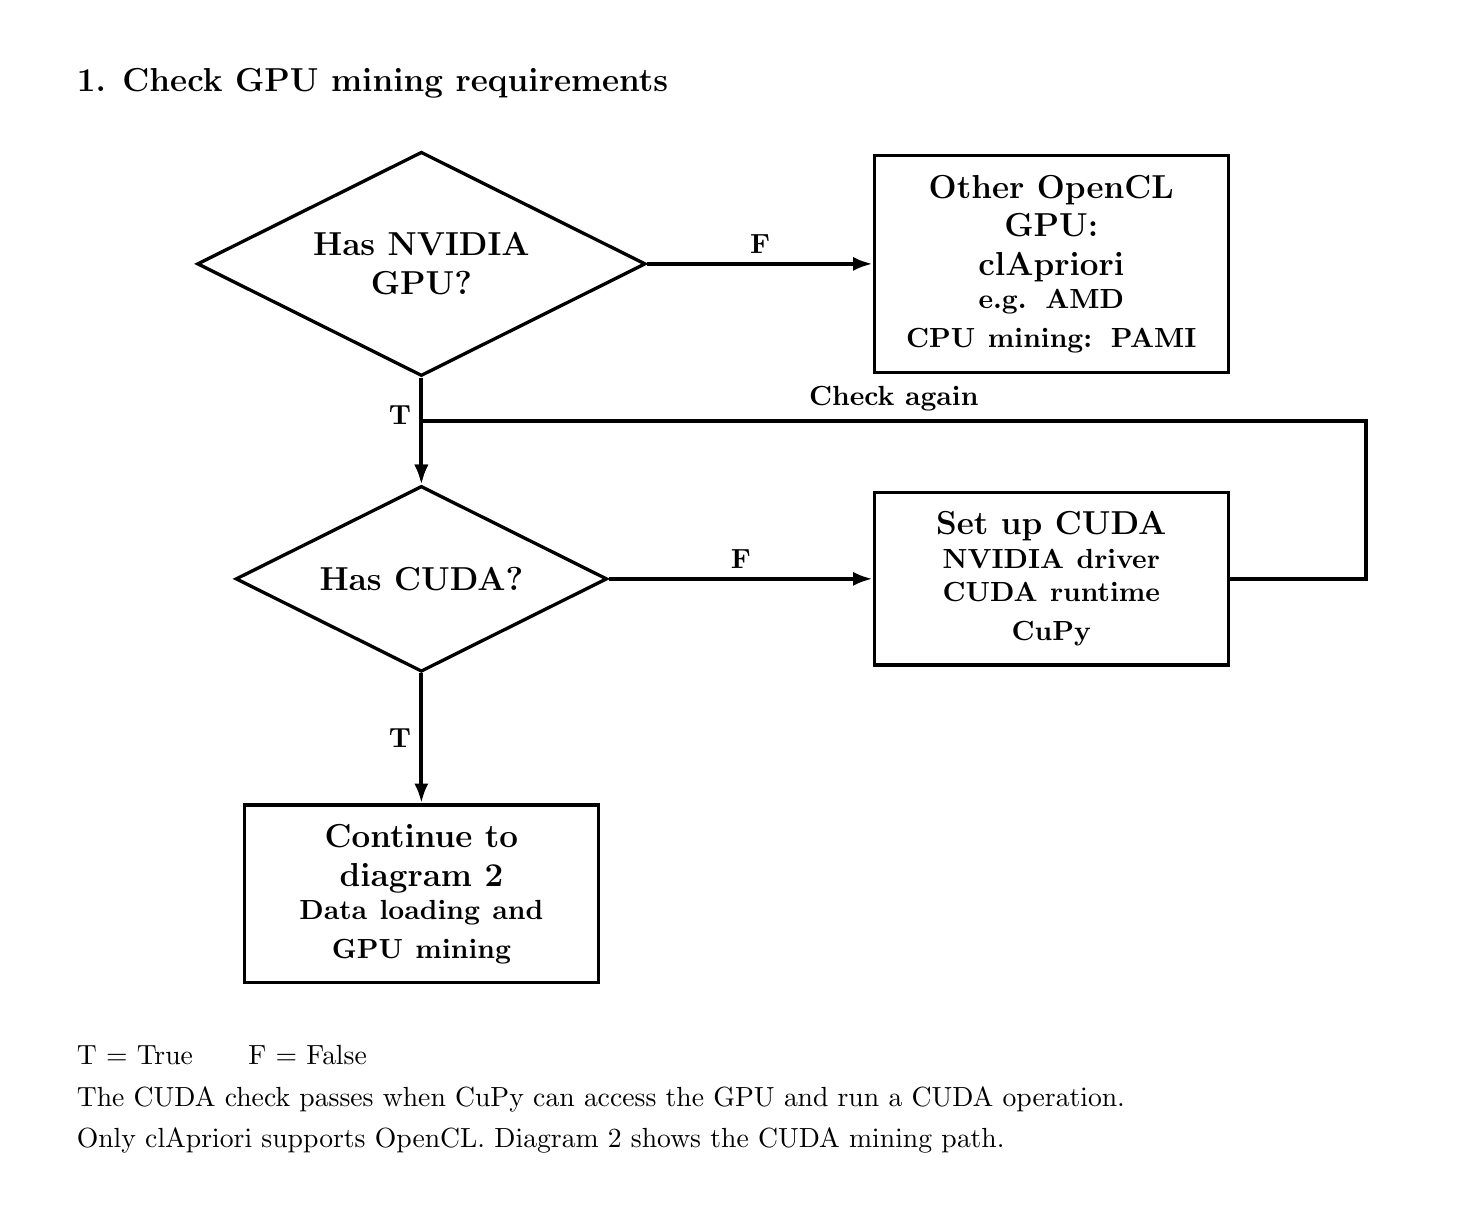
\begin{tikzpicture}[x=1cm,y=1cm,font=\large\bfseries,
 box/.style={draw=black,line width=1.2pt,fill=white,align=center,minimum height=1.4cm,text width=4cm,inner sep=7pt},
 question/.style={diamond,aspect=2,draw=black,line width=1.2pt,fill=white,align=center,text width=3.5cm,inner sep=3pt},
 flow/.style={-{Latex[length=2.5mm,width=1.8mm]},line width=1.4pt},
 label/.style={font=\normalsize\bfseries,fill=white,inner sep=3pt}]
\fill[white] (0,-4.6) rectangle (18,10);
\node[anchor=west,font=\large\bfseries] at (.5,9.3) {1. Check GPU mining requirements};

\node[question] (gpu) at (5,7) {Has NVIDIA\\GPU?};
\node[question] (cuda) at (5,3) {Has CUDA?};
\node[box] (ready) at (5,-1) {Continue to diagram 2\\\normalsize Data loading and\\GPU mining};
\node[box] (cpu) at (13,7) {Other OpenCL GPU:\\clApriori\\\normalsize e.g. AMD\\CPU mining: PAMI};
\node[box] (setup) at (13,3) {Set up CUDA\\\normalsize NVIDIA driver\\CUDA runtime\\CuPy};

\draw[flow] (gpu.south) -- node[label,left,pos=.35] {T} (cuda.north);
\draw[flow] (gpu.east) -- node[label,above] {F} (cpu.west);
\draw[flow] (cuda.south) -- node[label,left] {T} (ready.north);
\draw[flow] (cuda.east) -- node[label,above] {F} (setup.west);
\draw[flow] (setup.east) -- (17,3) -- (17,5) -- node[label,above] {Check again} (5,5) -- (cuda.north);

\node[anchor=north west,align=left,text width=16.5cm,font=\normalsize] at (.5,-2.8) {
T = True\qquad F = False\\[3pt]
The CUDA check passes when CuPy can access the GPU and run a CUDA operation.\\[3pt]
Only clApriori supports OpenCL. Diagram 2 shows the CUDA mining path.};
\end{tikzpicture}
\end{document}
